% \usepackage{hyperref}
% \hypersetup{
%     colorlinks=true,
%     linkcolor=blue,
%     filecolor=magenta,      
%     urlcolor=cyan,
% }

\question Construct a minimum spanning tree by running Prim's Algorithm from node A.\\

Break ties alphabetically: if you have the choice between two edges with the same weight, pick the one that has the smallest alphabetical vertex. If they both share a vertex, pick the one whose second vertex is smaller. Provide the ordering in which you broke ties, and order them alphabetically by vertex. For example if you break an edge between vertex Z and Y or vice versa, call it YZ.\\

%\begin{center}
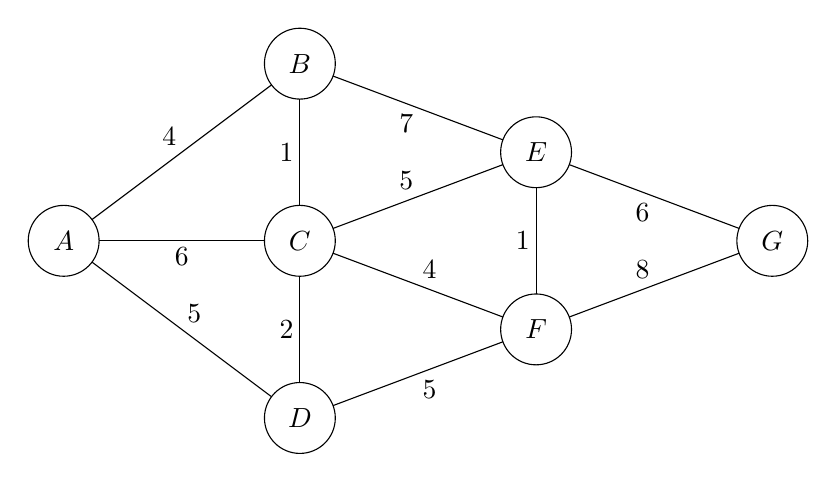
\begin{tikzpicture}[scale=0.15]
\tikzstyle{every node}+=[inner sep=0pt]
\draw (30,-15) circle (3);
\draw (30,-15) node {$B$};
\draw (10,-30) circle (3);
\draw (10,-30) node {$A$};
\draw (30,-30) circle (3);
\draw (30,-30) node {$C$};
\draw (30,-45) circle (3);
\draw (30,-45) node {$D$};
\draw (50,-37.5) circle (3);
\draw (50,-37.5) node {$F$};
\draw (50,-22.5) circle (3);
\draw (50,-22.5) node {$E$};
\draw (70,-30) circle (3);
\draw (70,-30) node {$G$};
\draw (27.6,-16.8) -- (12.4,-28.2);
\draw (18.94,-22) node [above] {$4$};
\draw (30,-18) -- (30,-27);
\draw (29.5,-22.5) node [left] {$1$};
\draw (13,-30) -- (27,-30);
\draw (20,-30.5) node [below] {$6$};
\draw (27.6,-43.2) -- (12.4,-31.8);
\draw (21.06,-37) node [above] {$5$};
\draw (30,-33) -- (30,-42);
\draw (29.5,-37.5) node [left] {$2$};
\draw (32.81,-43.95) -- (47.19,-38.55);
\draw (40.99,-41.77) node [below] {$5$};
\draw (47.19,-36.45) -- (32.81,-31.05);
\draw (40.99,-33.23) node [above] {$4$};
\draw (52.81,-23.55) -- (67.19,-28.95);
\draw (59.01,-26.77) node [below] {$6$};
\draw (67.19,-31.05) -- (52.81,-36.45);
\draw (59.01,-33.23) node [above] {$8$};
\draw (47.19,-23.55) -- (32.81,-28.95);
\draw (39.01,-25.73) node [above] {$5$};
\draw (50,-25.5) -- (50,-34.5);
\draw (49.5,-30) node [left] {$1$};
\draw (32.81,-16.05) -- (47.19,-21.45);
\draw (39.01,-19.27) node [below] {$7$};
\end{tikzpicture}
%\end{center}

%\begin{parts}
\begin{solution}
See walkthrough slides \href{https://docs.google.com/presentation/d/1fhQAlA94zKMbf-vBcTL-MZY8B1-l9ERV1qfCZcNS764/edit#slide=id.gab8a60590f_0_0}{here}.

Ordering is AB, BC, CD, CF, EF, EG

%\begin{center}
\begin{tikzpicture}[scale=0.15]
\tikzstyle{every node}+=[inner sep=0pt]
\draw (30,-15) circle (3);
\draw (30,-15) node {$B$};
\draw (10,-30) circle (3);
\draw (10,-30) node {$A$};
\draw (30,-30) circle (3);
\draw (30,-30) node {$C$};
\draw (30,-45) circle (3);
\draw (30,-45) node {$D$};
\draw (50,-37.5) circle (3);
\draw (50,-37.5) node {$F$};
\draw (50,-22.5) circle (3);
\draw (50,-22.5) node {$E$};
\draw (70,-30) circle (3);
\draw (70,-30) node {$G$};
\draw (27.6,-16.8) -- (12.4,-28.2);
\draw (18.94,-22) node [above] {$4$};
\draw (30,-18) -- (30,-27);
\draw (29.5,-22.5) node [left] {$1$};
\draw (30,-33) -- (30,-42);
\draw (29.5,-37.5) node [left] {$2$};
\draw (47.19,-36.45) -- (32.81,-31.05);
\draw (40.99,-33.23) node [above] {$4$};
\draw (52.81,-23.55) -- (67.19,-28.95);
\draw (59.01,-26.77) node [below] {$6$};
\draw (50,-25.5) -- (50,-34.5);
\draw (49.5,-30) node [left] {$1$};
\end{tikzpicture}
%\end{center}

\textbf{Meta}:\newline 
Intro: The cut property is introduced in the general statement for this question. Make sure to have a simple example to use as a visual when explaining it to students.\\
1.3: Your board work for how to run through Prim's should be very similar to how you ran through Djikstra's algorithm in the previous worksheet. Only add edges to your MST as you pop off the Fringe (PQ). Additionally, after running through the problem, explain how at a high level, for every edge added, we just added the shortest edge not in the MST into the MST. Use the cut property to explain this.
\end{solution}
%\end{parts}
